\documentclass[]{../template/Report}%方括号内写yuxi即生成预习报告\documentclass[yuxi]{../template/Report}
\settemplatedir{../template/}%设置模板路径

\exname{等厚干涉} %实验名称
\extable{14} %实验桌号
\instructor{张利} %指导教师
\class{信工2401} %班级
\name{姚舜瑜} %姓名
\stuid{3240100532} %学号

\nyear{2025} %年
\nmonth{12} %月
\nday{2} %日
\nweekday{二} %星期几，e.g. \nweekday{三}
\daypart{上午}%上午/下午

\redate{} %如有实验补做，补做日期
\resitu{} %情况说明：

\begin{document}
\maketitle%输出封面

\section{预习报告（10分）}
\subsection{实验综述（5分）}

\subsubsection{实验目的}
\begin{enumerate}
  \item 通过观察牛顿环和劈尖干涉条纹，直观熟悉等厚干涉现象，理解膜厚与条纹级次之间的对应关系。
  \item 学会利用牛顿环测量凸透镜曲率半径、利用劈尖条纹测量薄片厚度的基本步骤和数据处理方法。
  \item 练习读数显微镜的使用，体会单向读数、减小空程误差和估计不确定度在精密测量中的作用。
\end{enumerate}

\subsubsection{背景与原理}
等厚干涉是一种经典的光学干涉现象，产生于两块光滑透明介质之间的薄膜。当单色光近垂直入射时，薄膜中不同位置的膜厚决定了反射光的光程差，从而形成明暗相间的干涉条纹。由于膜厚在空间上分布不均匀，不同位置对应不同的干涉级次，形成等厚干涉图样。

本实验属于反射式等厚干涉：两光滑界面之间形成的薄膜中，只要局部膜厚相同，反射光的光程差就相同，从而得到同一级条纹。近垂直入射单色光时，上下表面反射光的光程差为
\[
\Delta = 2e + \frac{\lambda}{2},
\]
其中 $e$ 为膜厚，$\lambda/2$ 表示一次反射导致的半波相位变化。反射暗纹满足
\[
\Delta = k\lambda,\quad k=0,1,2,\dots
\]

以此为基础，便可以解释两种典型的等厚干涉现象：牛顿环与劈尖干涉。并根据理论推理和测量结果得到目标物理量。

\paragraph{\textbf{1. 牛顿环：}}
\paragraph{}
将曲率半径为 $R$ 的凸透镜轻放在平板玻璃上，在接触附近形成很薄的空气层。几何关系表明，当 $r\ll R$ 时，距中心半径为 $r$ 处的空气层厚度近似
\[
e \approx \frac{r^2}{2R},
\]
代入暗纹条件可得第 $k$ 级暗环
\[
r_k^2 = kR\lambda.
\]
因此 $r_k^2$ 与条纹级次 $k$ 近似成线性关系。实际处理中常取两级暗环平方差
\[
r_m^2 - r_n^2 = (m-n)R\lambda,
\]
从而计算
\[
R = \frac{r_m^2 - r_n^2}{(m-n)\lambda}
  = \frac{\Delta d^2}{4(m-n)\lambda},
\]
以减弱中心定位和单次读数误差的影响。


\paragraph{\textbf{2. 劈尖干涉：}}
\paragraph{}

用两块玻璃片与待测薄片在一端组成空气劈尖，沿劈尖方向膜厚近似线性变化。相邻同种条纹对应的膜厚差约为 $\lambda/2$。若在长度为 $L$ 的一段劈尖上共数到 $N$ 条条纹，则薄片厚度
\[
e = \frac{\lambda N}{2} = \frac{\lambda nL}{2},
\]
其中 $n$ 为单位长度内的条纹条数。为减小读数误差，通常利用跨越 10 条纹的平均条距
\[
\overline{\Delta S}_{10} = \frac{1}{10}\sum_{i=1}^{10}(S_{i+10} - S_i),\quad
n = \frac{10}{\overline{\Delta S}_{10}},
\]
于是得到
\[
e = \frac{50L\lambda}{\sum_{i=1}^{10}(S_{i+10} - S_i)}.
\]
最终结果写成 $e = \bar e \pm u_e$ 的形式，并说明主要不确定度来源。

\begin{figure}[H]
  \centering
  \begin{minipage}{0.45\textwidth}
    \centering
  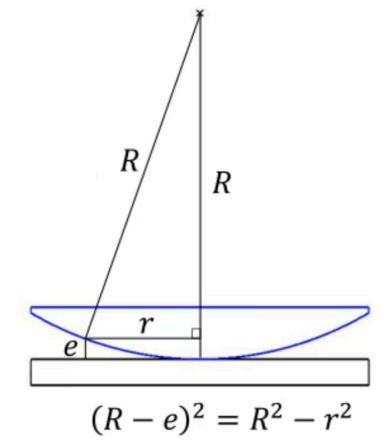
\includegraphics[width=0.8\textwidth]{figures/仪器示意图.png}
  \caption{牛顿环原理示意图}
  \end{minipage}
  \hfill
  \begin{minipage}{0.45\textwidth}
    \centering
  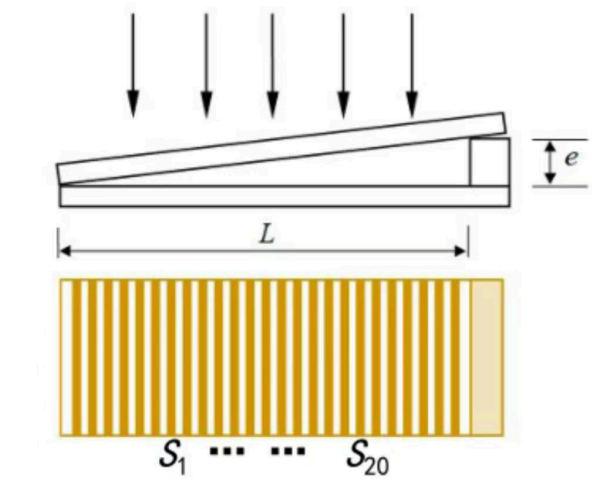
\includegraphics[width=\textwidth]{figures/条纹示意图.png}
  \caption{劈尖干涉原理示意图}
  \end{minipage}
\end{figure}
\subsubsection{实验仪器}
钠灯；读数显微镜；光学平板玻璃和凸透镜（牛顿环装置）；两块平玻璃片与待测薄片（劈尖干涉装置）；半反半透镜等。

\subsubsection{实验内容}
\begin{enumerate}
  \item \textbf{读数显微镜调节：}先调节目镜使十字丝清晰，再调物镜使条纹成像锐利，移动视线检查并消除视差。
  \item \textbf{牛顿环实验：}搭建牛顿环装置，调整透镜与平板的接触和水平度，使同心环清晰。用读数显微镜沿固定方向单向转动测微鼓轮，记录若干级左右暗环位置，计算各级半径 $r_k$，建立 $r_k^2$–$k$ 关系，拟合得到凸透镜曲率半径 $R$。
  \item \textbf{劈尖测厚实验：}搭建劈尖干涉装置，微调劈尖角度和显微镜焦距，使直条纹细而清晰。选取包含薄片的一段长度 $L$，多次记录条纹坐标（如 $S_i$ 与 $S_{i+10}$），求出平均条距和条纹密度 $n$，代入公式计算薄片厚度，并结合重复测量结果估算不确定度。
\end{enumerate}

\subsection{实验重点（3分）}

\begin{itemize}
  \item 理解等厚干涉原理，掌握牛顿环和劈尖干涉的形成机制及其与膜厚的关系。
  \item 熟练使用读数显微镜，掌握单向读数和减小空程误差的方法。
  \item 能结合实验数据进行合理的数据处理和不确定度分析。
\end{itemize}

\subsection{实验难点（2分）}

\begin{itemize}
  \item 牛顿环中心及高阶条纹对比度较低，中心位置与条纹级次判定容易产生偏差。
  \item 读数显微镜存在回程间隙，若未严格单向读数，易引入系统性空程误差。
  \item 劈尖条纹细密，对显微镜对焦、劈尖平行度和光路垂直度要求较高，稍有偏差就会导致条纹模糊、计数困难。
\end{itemize}
\begin{fullreportonly}
\section{原始数据（20分）}
\begin{figure}[H]
  \centering
  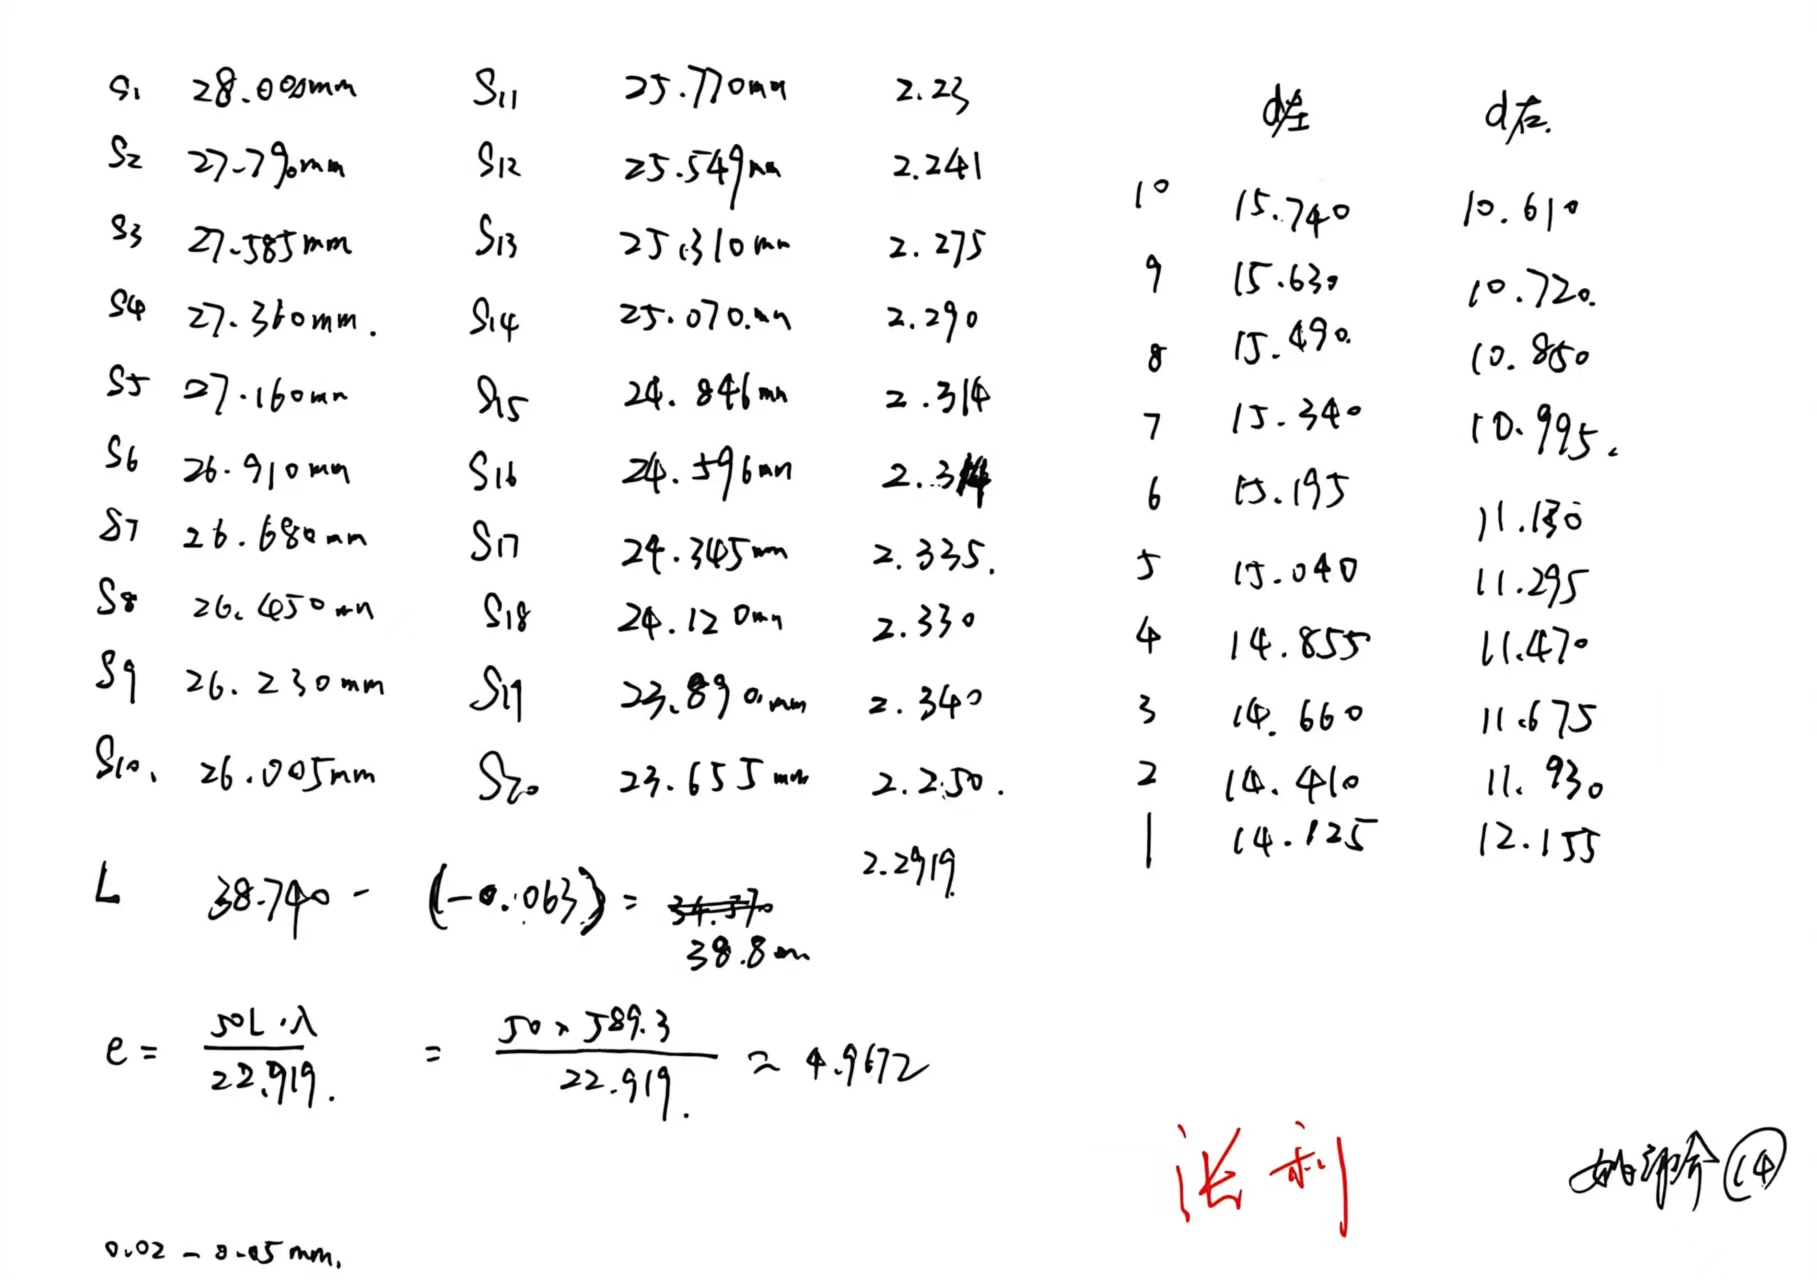
\includegraphics[width=0.8\textwidth]{figures/Y原始数据.jpg}
  \caption{实验原始数据记录示例}
\end{figure}
\newpage
\section{结果与分析（60分）}
\subsection{数据处理与结果（30分）}
\subsubsection{牛顿环实验结果}

\subsubsection{劈尖干涉实验结果}

\subsection{误差分析（20分）}
（运用测量误差、相对误差或不确定度等分析实验结果，写出完整的结果表达式，并分析误差原因。）

\subsection{实验探讨（10分）}
（对实验内容、现象和过程的小结，不超过100字。）

\section{思考题（10分）}
（解答教材或讲义或老师布置的思考题，请先写题干，再作答。）
\end{fullreportonly}
\insertnotes
\end{document}